\subsection{Vehicle Dynamics}
\label{sect:vehicle-dynamics}
The \emph{ego vehicle} is the agent whose actions we wish to verify. Clearly, there are a variety of levels of abstraction which such an agent can be modeled at. Fig. \ref{fig:abstraction} details the different levels of abstraction which the ego vehicle may be interogated at...

\begin{figure}
	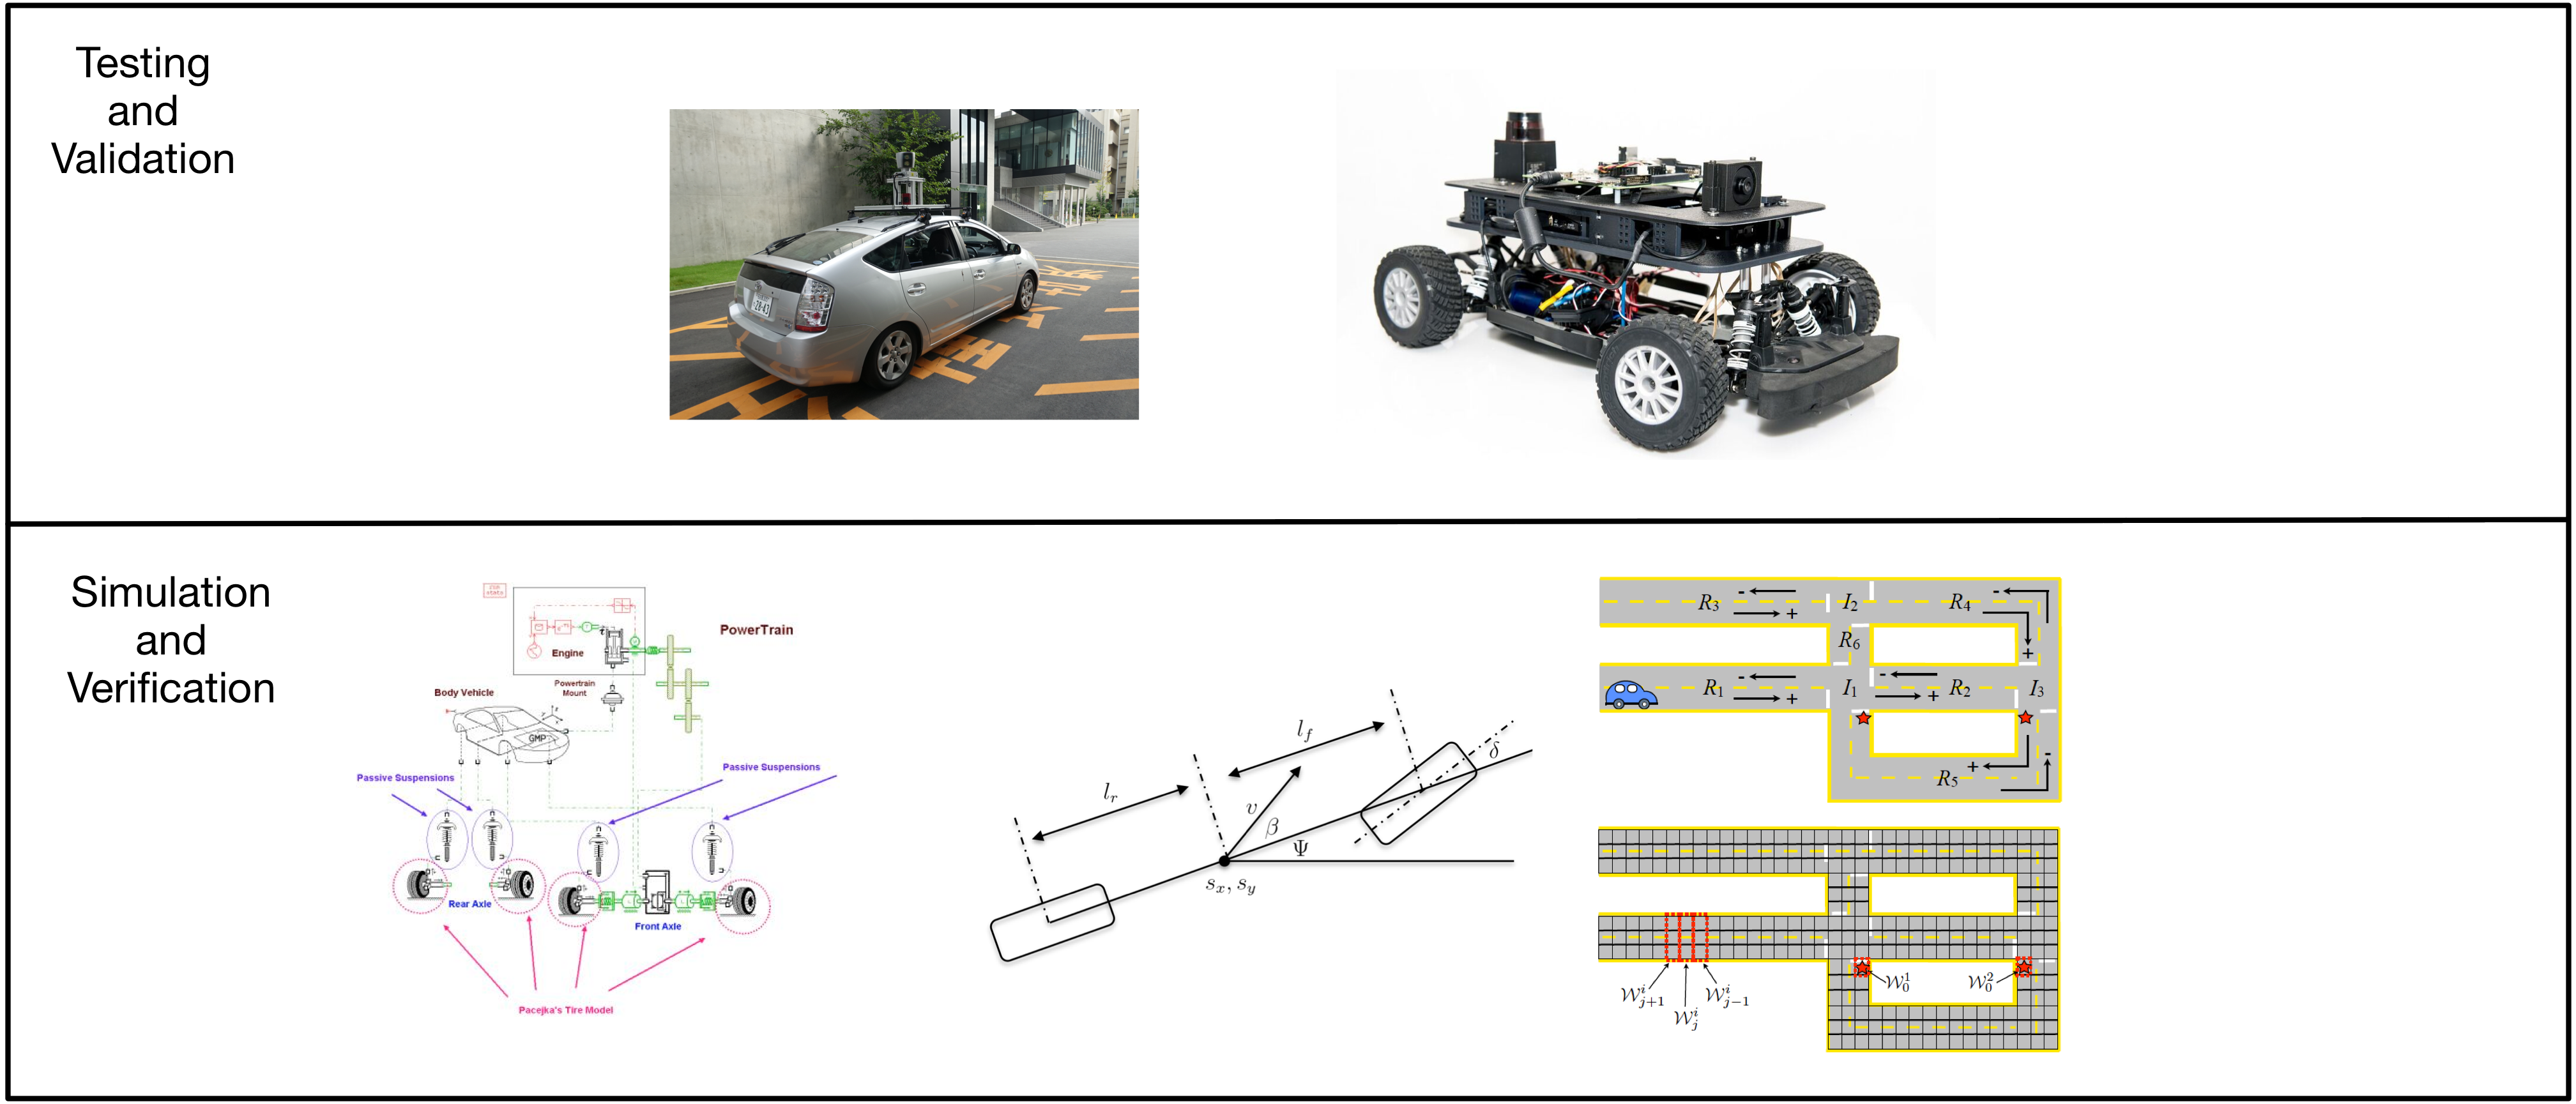
\includegraphics[width=\textwidth]{figures/abstraction}
	\caption{Levels of ego-vehicle abstraction. Goldilocks problem, expressive enough to capture relevant properties, but simple enough to be tractable}
	\label{fig:abstraction}
\end{figure}
APEX uses a non-linear 7 dimensional bicycle model \cite{Rajamani2011} in order to describe the ego-vehicle. This abstraction is common in control theoretic design methodologies. It preserves the relationship between higher level planning activities such as trajectory generation and lower level controllers which actuate the steering mechanism, acceleration, and braking. 

See Fig. \ref{fig:bike}. 
The input to such a model is steering angle velocity and linear velocity, the output is vehicle state as a function of time. These inputs are computed by the trajectory tracking controllers outlined in Section \ref{sect:tracking}

\begin{figure}
	\centering
	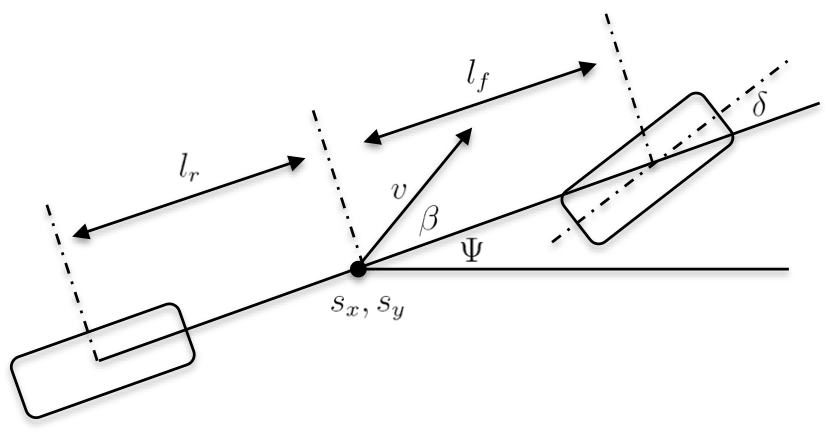
\includegraphics[scale=.75]{figures/bicycle_model}
	\caption{Nonlinear bicycle model describing the statespace for the APEX approach to vehicle dynamics}
	\label{fig:bike}
\end{figure}

The state vector describing the vehicle is described in equations (1)-(7). 
The variable \(\beta\) is the slip angle at the center of mass, \(\psi\) is the heading angle, \(\dot{\psi}\) is the yaw rate, \(v\) is the velocity, \(s_x\) and \(s_y\) are the x and y positions, and \(\delta\) is the angle of the front wheel. In the formulation of [6], the inputs to the system are \(a_x\), the longitudinal acceleration, and \(v_w\) the rotational speed of the steering angle. 
%The \(y\) terms represent disturbances to the system. For example \(y_{\beta}\) and \(y_{\dot{\psi}}\) represent disturbances to the slip angle at the center of mass and the yaw rate. 
\begin{equation}
x_v = (\beta,\Psi,\dot{\Psi}, v, s_x, s_y, \delta)
\end{equation}	
The state equations for the system as described in \cite{Althoff2014} are:
\begin{equation}
\label{eqn:beta}
\dot{\beta}=\left(\frac{C_rl_r-C_fl_f}{mv^2} \right)\dot{\psi}+\left(\frac{C_f}{mv} \right)\delta-\left(\frac{C_f+C_r}{mv} \right)\beta
\end{equation}
\begin{gather}
\label{eqn:psi}
\ddot{\psi}=\left(\frac{C_rl_r-C_fl_f}{I_z} \right)\beta-\left(\frac{C_fl_f^2-C_rl_r^2}{I_z} \right)\left(\frac{\dot{\psi}}{v} \right) \notag \\
+\left(\frac{C_fl_f}{I_z} \right)\delta
\end{gather}
\begin{equation}
\label{eqn:v}
\dot{v}=a_x
\end{equation}
\begin{equation}
\label{eqn:sx}
\dot{s_x}=v\cos{(\beta+\psi)}
\end{equation}
\begin{equation}
\label{eqn:sy}
\dot{s_y}=v\sin{(\beta+\psi)}	
\end{equation}	
\begin{equation}
\label{eqn:delta}
\dot{\delta}=v_w
\end{equation}